\subsection{Unlocking the Mystery: The Role of a Beverage Antenna's Termination Resistor!}

\begin{tcolorbox}[colback=gray!10, colframe=black, title=E9H07] What is the function of a Beverage antenna’s termination resistor?
\begin{enumerate}[label=\Alph*.]
    \item Increase the front-to-side ratio
    \item \textbf{Absorb signals from the reverse direction}
    \item Decrease SWR bandwidth
    \item Eliminate harmonic reception
\end{enumerate} \end{tcolorbox}

\subsubsection{Concepts Related to Beverage Antennas}
Beverage antennas are a type of receiving antenna that is widely used in low-frequency (LF) and very low-frequency (VLF) communication. They are particularly known for their ability to receive weak signals, making them favored among amateur radio operators and shortwave listeners. 

The termination resistor plays a critical role in the performance of Beverage antennas. Its primary function is to absorb signals that arrive from the reverse direction, thus minimizing reflections and improving the overall antenna's performance.

\subsubsection{Understanding Termination Resistors}
A Beverage antenna typically consists of a long wire suspended above the ground. The direction of maximum reception is determined by the orientation of the wire. To improve directional reception and reduce noise, a termination resistor is placed at the end of the antenna opposite to the feed point.

When the termination resistor is correctly matched to the characteristic impedance of the antenna (usually around 300 ohms), it effectively absorbs incoming signals that come from behind the antenna (the reverse direction). This process minimizes unwanted reflections, which can lead to signal distortion and loss.

\subsubsection{Summary of Key Concepts}
1. \textbf{Antenna Directivity:}: Beverage antennas are designed to be directional, favoring signals arriving from the front.
2. \textbf{Termination Resistors:}: They are used to absorb signals from undesired directions, improving signal clarity.
3. \textbf{Impedance Matching:}: Matching the termination resistor to the antenna's impedance is essential for optimal performance.

If you have further questions or need additional clarifications regarding the principles behind Beverage antennas or the function of termination resistors, please feel free to ask.

\begin{center}
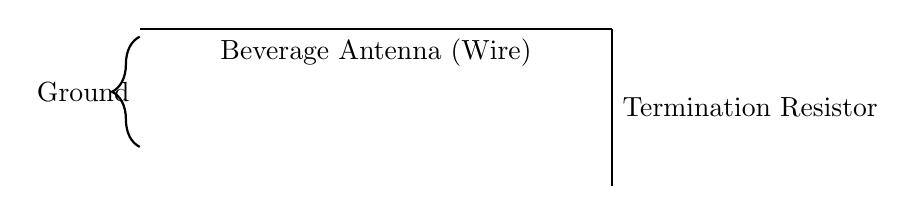
\begin{tikzpicture}
    % Draw a simple Beverage antenna configuration
    \draw[thick] (0,0) -- (6,0) node[midway, below] {Beverage Antenna (Wire)};
    \draw[thick] (6,0) -- (6,-2) node[midway, right] {Termination Resistor};
    
    % Add ground
    \draw[thick,decorate,decoration={brace,amplitude=10pt,mirror}] (0,-0.1) -- node[midway,left]{Ground} (0,-1.5);
\end{tikzpicture}
\end{center}
